\section{Introduction}

The audible world holds much information, often information that we as humans either cannot hear or ignore in favor for other sensory cues. Through audio alone, models have been able to accurately determine the inner state of an animal or other human, a task in which often accomplished through visual cues \cite{Farago2010, schuller_acoustic_2009}. Additionally, the environment characteristics are able to be accurately determined without the aid of visual cues \cite{Eronen2006}. In human speech, speaker discrimination is also possible and has found its way into several intelligent assistants \cite{Campbell1997}. Finally, perhaps the best known and most widely studied application for audio is obtaining textual representations of speech \cite{Rabiner1989}. These applications are unlikely the limit of what we can glean from audio data and with audio recording devices becoming more ubiquitous and cheaper than imagery collection, we are obtaining more audio from a wider variety of places.

Over the last decade, audio has become easier to collect in environments ranging from in-home microphones in intelligent assistants to wearable devices in an ocean setting \cite{kohlsdorf_underwater_2013}. This is in part a consequence of embedded systems becoming smaller and more efficient as well as improvements in the quality of small microphones. It has become feasible to collect quality audio data from mobile phones and wearables able to record throughout the day \cite{Lane2015, Choudhury2008}. However with this increase of audio sources, more audio than ever is being collected.

Fortunately, the cost of data storage is low and looks to continue to become cheaper. Though as the amount of data increases, the number of man-hours required to label it increases along with it. Also, when manually labeling large datasets data can be mislabeled or overlooked entirely \cite{Bardeli2009, Rong2018}. Often with large datasets, content-based retrieval techniques are used to allow researchers to label a small subset of the dataset and be presented with statistically significant examples they may have previously missed.

Content-based retrieval is a method of querying information from an unstructured dataset. Before the advent of \textit{Big Data}, naive approaches like similarity search retrieved desired information in an acceptable time frame. Similarity search in audio uses exemplars of a document to find other matches in the dataset. This approach is restrictive in two ways. First, it requires an exemplar of all desired audio segments which can at times defeat the purpose of searching the dataset and doesn't allow for easy dataset exploration. Second, it must check similarity of every file in the dataset which requires a significant amount of time even with efficient algorithms. Today, the datasets are much too large to use naive approaches and thus require more nuanced methods and compact data representations to be useful to users.

Content-based retrieval has been investigated thoroughly in image datasets with much success. However, attempts to apply these image techniques to audio spectrograms have seen mixed success. This is in large part due to the "transparency" of audio where if multiple audio sources exist in the data, they can overlap in similar frequency ranges. Thus we investigate using a different audio representation and probabilistic retrieval for exploration of audio datasets.

Here, I propose creating a model based on a taxonomy of human audio perception. As mentioned before, audio signals can contain a large amount of information but this information is mostly from combinations of the low level intensity, spectral, and statistical properties. These properties form the base of a hierarchical representation of sound that is combined to form temporal properties which then are made into cognitive properties. Perception is of interest as the human capacity continues to exceed that of machine listeners, thus it is hypothesized better performance can be gained from understanding and modelling human systems. This hypothesis has led to psychological and physiological studies into how and why human perception is accurate and how it audio can be optimally encoded \cite{Gaver1993, Eggermont2001, slaney1993importance, Piazza2013}.

In all, the contributions this work provides is as follows:
\begin{itemize}
    \item Present an audio representation based on human perception of sound.
    \item Demonstrate a model developed to match the Gaver taxonomy of sound.
    \item Use probabilistic models to retrieve unstructured data with high confidence.
\end{itemize}

\section{Background}
\begin{itemize}
    \item Machine Hearing Principles
    \item Spectrogram Based Machine Hearing
    \item Case for Audio-Based Machine Hearing (w/ results teaser)
\end{itemize}

\subsection{Machine Hearing Principles}

Much like computer vision, machine hearing is a field attempting to give autonomous agents the ability to use a sense in much the same way as humans. However, this field has lagged behind computer vision due to its seeming lack of general applicability. This is shown by the wealth of specialized music and speech sound analyses, with more general problems being ignored. Thus, machine hearing is less the study of recognizing specific events in audio but instead what representations and structures allow for a generalized model of sound. Lyon argues for a specific structure to machine hearing systems with four parts \cite{lyon_machine_2010}.

The first module is a peripheral analyzer, based on the \textit{cochlea} as most other outer-ear structures are at the mercy of the recording medium (e.g. the microphone). The \textit{cochlea} is responsible for forming sound representations. The \textit{cochlea} is responsible for converting acoustics into neural signals. It is a coiled tube separated by two membranes, the \textit{Reissner's membrane} and the \textit{basilar membrane} \cite{Plack2018}. Simply, the \textit{basilar membrane} can be considered as a collection of band-pass filters, separating sounds into spectral components. These components are then processed by brain structures that convert the waveform representation to something more usable.

This next module is where a large portion of the final representation is formed. It creates image representations of the audio, modeling the concept of \textit{echoic memory}. The perception of sound depends on what comes before and occurs after a sample of audio. Thus memory in this domain is important to perception. \textit{Echoic memory} is the name given to human auditory sensory memory. It is critical in permitting listeners to integrate incoming information with past events. However, among the literature there is some disagreement on the duration of the memory with some arguing ~250 ms and others ~4 seconds \cite{Wingfield2016}. Though it is difficult to achieve good results with only the image representation, and as such another module is often used to extract features.

A feature extraction module is then used to pull a compact and meaningful representation from the images formed in the previous module. This module most closely matches the \textit{neural code} of human audio perception which form the interface between the sound and its conscious perception. It should be noted, the human processing chain is still mostly unknown and much of what we do know is speculative. Though, it is hypothesized that multiple processes occur in sequence to prepare the information for perception \cite{Eggermont2001}. It is likely these processing steps make actual perception less computationally expensive. The outcome of this module is likely the most important as it determines the performance and efficiency of the decision module.

The decision module takes in the representation formed by the previous modules and maps it to some decision needed to be made. This module is analogous to conscious perception in humans. It can vary between very simple like a single perceptron to very complex like a deep neural network.

\subsection{Spectrogram-Based Machine Hearing}
\begin{itemize}
    \item How this fits into Neural Coding and Echoic Memory
    \item CNN approach
    \item Image retrieval (PAMIR approach)
\end{itemize}

Due to the good performance of content retrieval systems in the visual domain, several researchers attempted to use these approaches in the audio domain. This approach combines the neural coding and echoic memory portions of hearing. Instead of having a separate feature extraction module, a model is trained directly on the spectral image.

\begin{figure}[!tbp]
    \centering
    \subfloat[Noisy]{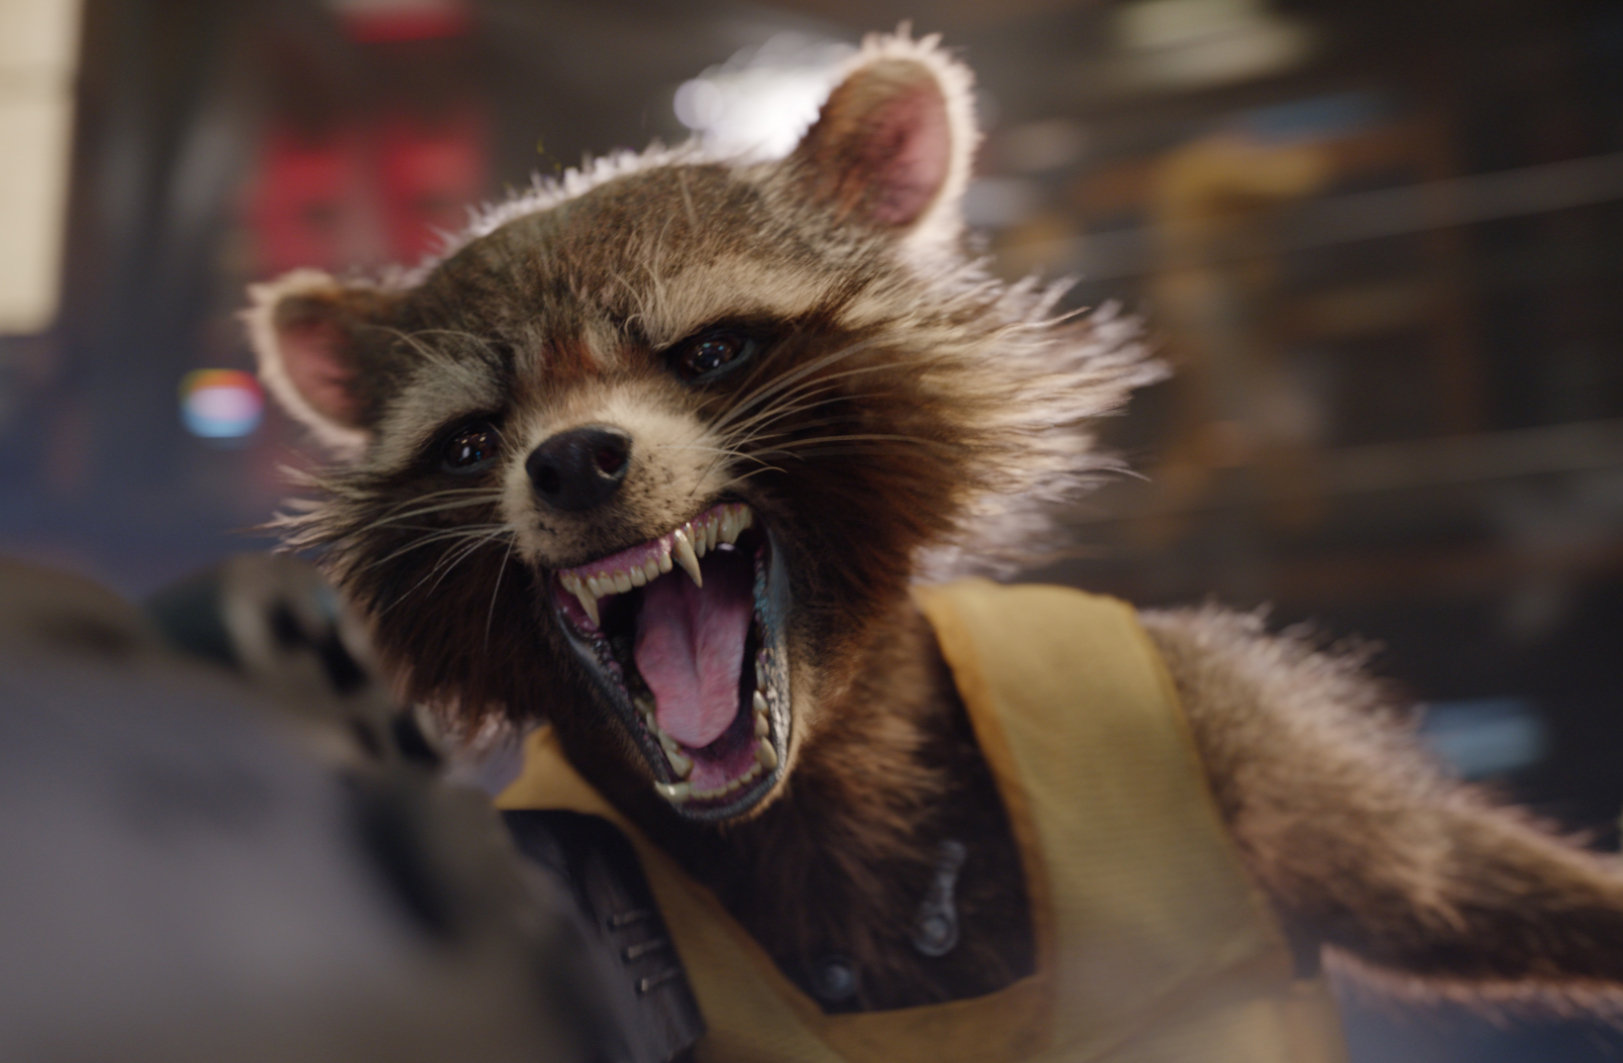
\includegraphics[width=0.4\textwidth]{figures/noisy_audio.jpg}\label{fig:noisy_audio}}
    \hfill
    \subfloat[Clean]{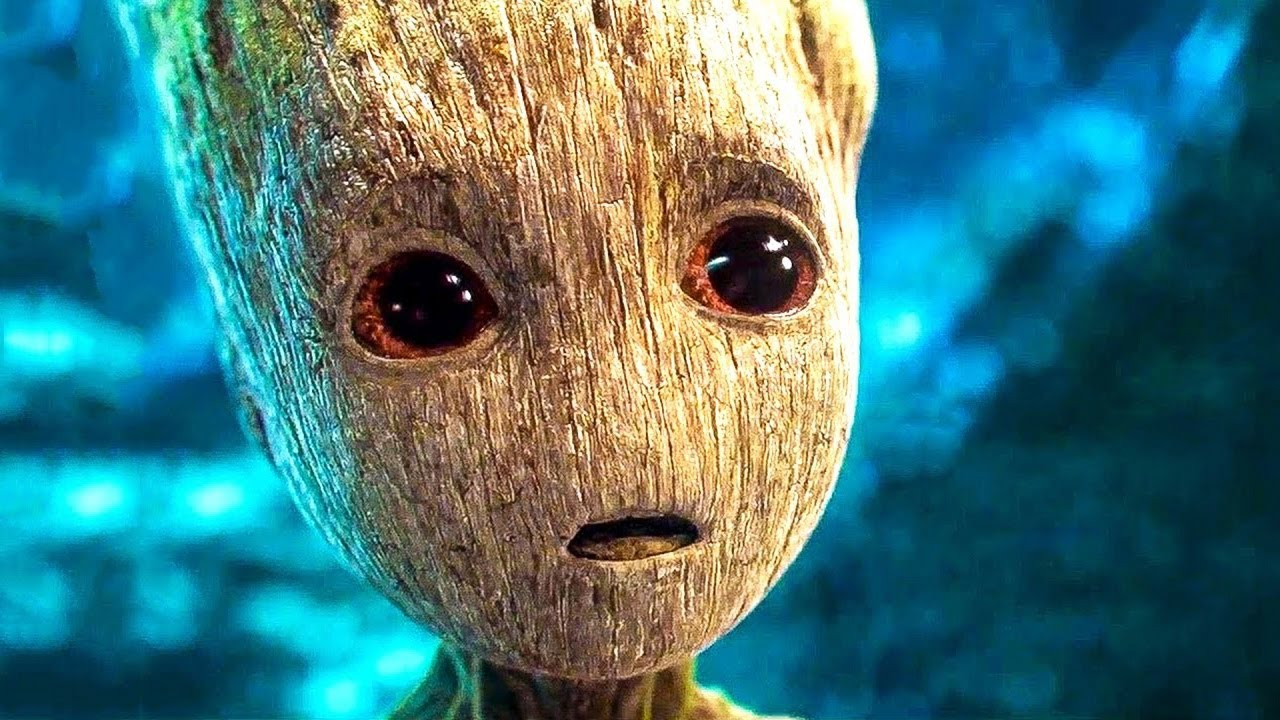
\includegraphics[width=0.4\textwidth]{figures/clean_audio.jpg}\label{fig:clean_audio}}
    \caption{Spectrograms illustrating the difference between clean and noisy audio when converted to visual domain.}
    \label{fig:noisy_audio_cmpr}
\end{figure}

Translating audio to a visual domain has seen some success, especially in cases where audio events are isolated as represented in \ref{fig:noisy_audio_cmpr}. Unfortunately in real-world situations, audio recordings usually have multiple audio sources in them often with overlapping frequencies. This is due to the "transparency" of audio, with spectral images being analogous to placing several transparent photos over one another. A Convolutional neural network is the most often applied learner for image classification and as such has often been applied to spectrogram images. However, these approaches struggle to break 70\% accuracy even with complex ensembles of networks \cite{xu_large-scale_2018, piczak_environmental_2015}.

In an attempt to capitalize on image retrieval success, Chechik et al. used spectrogram imagery to perform unstructured audio retrieval with passive-aggressive model for image retrieval (PAMIR) \cite{Chechik2008}. This work used probabilistic confidence to rank audio documents on relevance to a text query. When tested against the Freesound dataset though it saw no improvement over GMM or SVM using traditional audio features. The average precision of the classifier was 0.27 with a max of about 0.55.

\subsection{Waveform-Based Machine Hearing}
\begin{itemize}
    \item Audio features + how they apply
    \item RNN approaches
    \item My approach + some teaser
\end{itemize}

\section{Pipeline Overview}

\begin{figure}[!h]
    \centering
    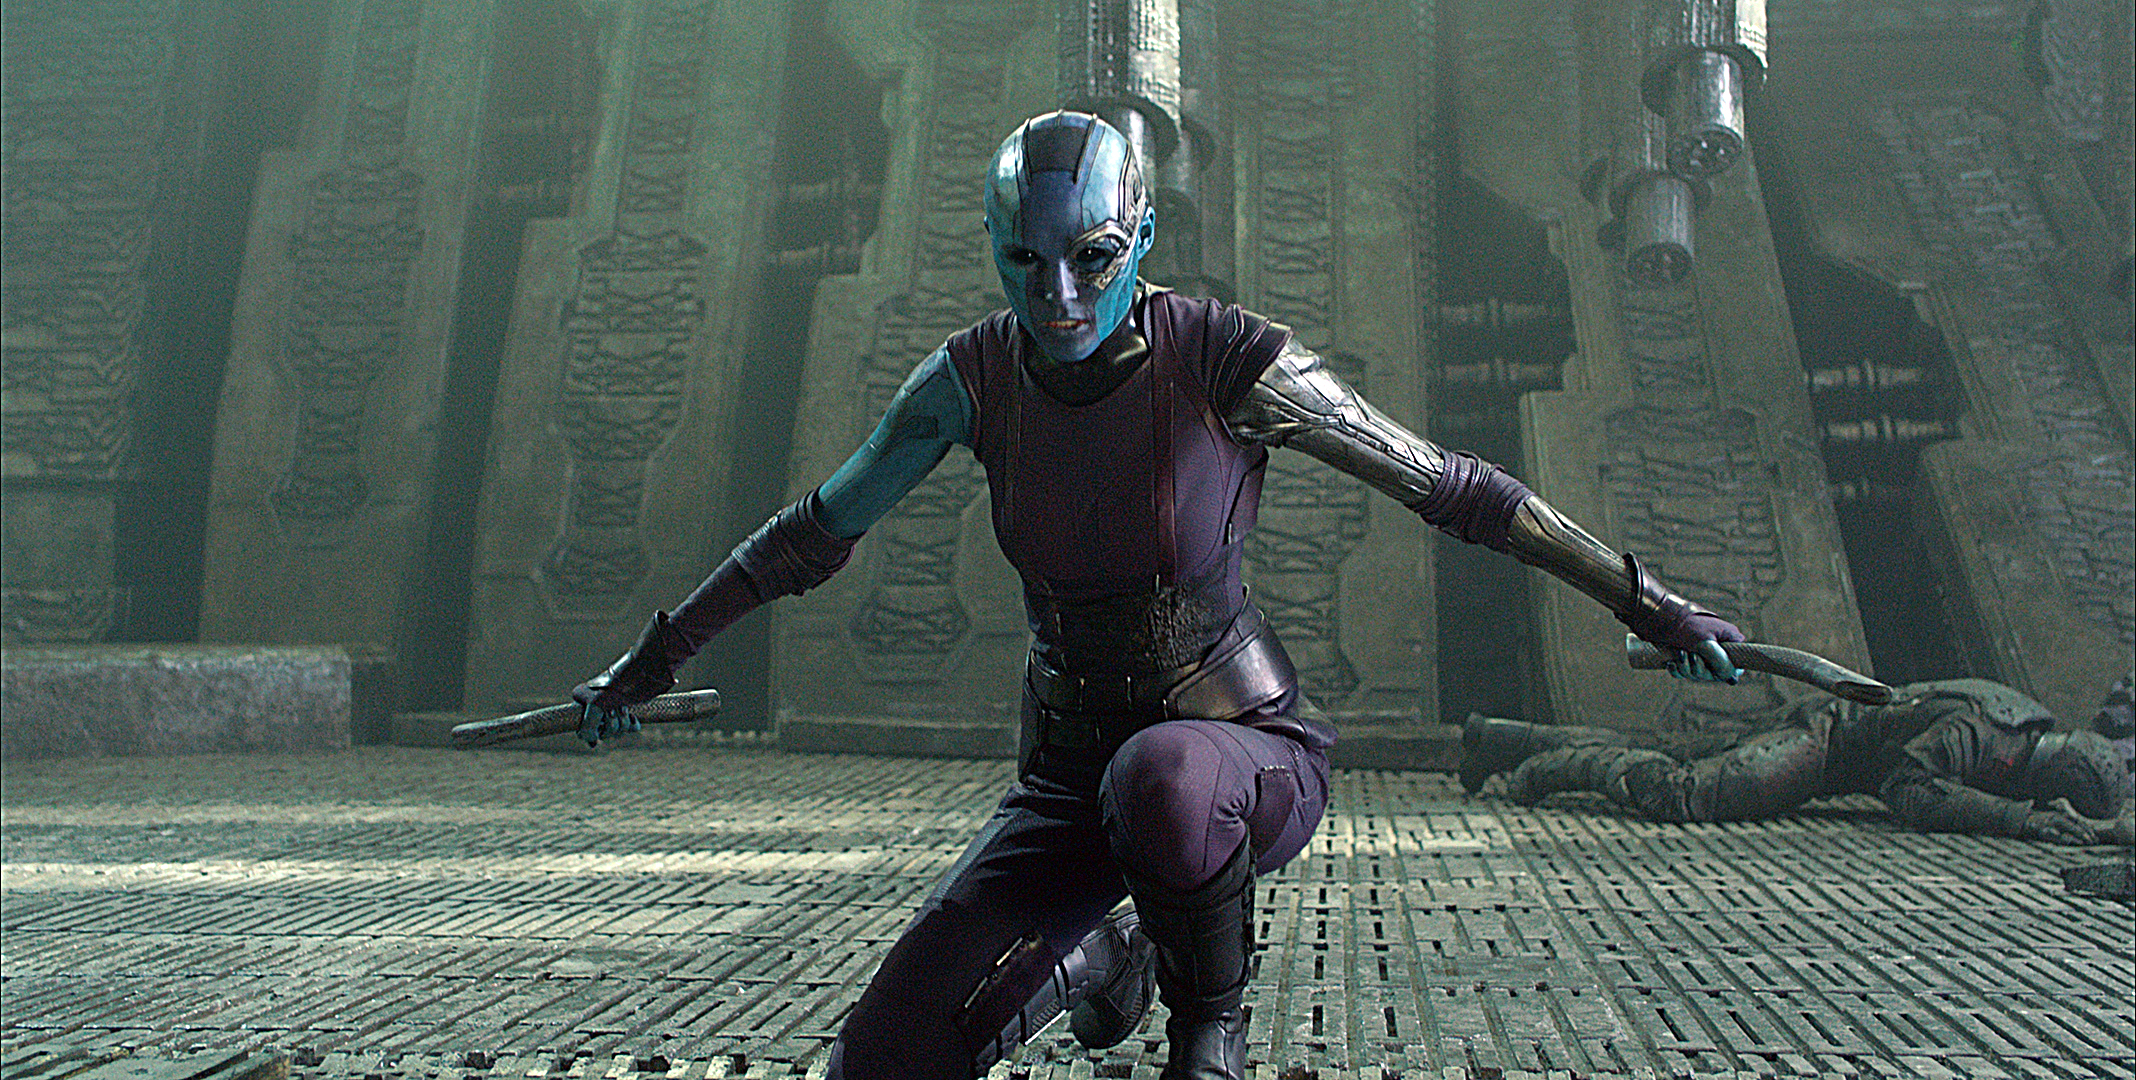
\includegraphics[width=0.49\textwidth]{figures/pipeline.jpg}
    \caption{Pipeline for the proposed approach}
    \label{fig:pipeline}
\end{figure}

This approach closely follows Lyon's structure of machine hearing systems. Audio goes through each stage sequentially with portions of it optimized for parallel execution. The pipeline first converts the waveform to a gammatone spectrogram of a given time window. Features are then extracted from this representation using standard extraction techniques to get a combination of spectral and temporal features. Finally, a hierarchical ensemble of probabilistic classifiers is trained to create the model.

\subsection{Acoustic Features}
First in the classification pipeline is an encoding of audio signals. Each audio file in the dataset is read in blocks of time with overlapping segments in an effort to have the data cover all audio objects. Blocks with no sound are discarded, this is done to reduce data size but also to avoid correlating silence to some class which can easily confuse the agent. Each block of audio then has its spectrogram computed from which the frequency features are extracted. In addition to the frequency features, temporal statistics of the raw audio is used to capture temporal properties of the signal. An LSTM auto-encoder is also used to extract relevant features from the spectrogram as described by Meyer \cite{Meyer2017}.

\subsection{Classification Model}

The proposed classification model is illustrated in Figure ~\ref{fig:NetHier}. At the top level are the most general descriptors of a sound and are thought to be easily classified. A shallow neural network is used to allow the most obviously unrelated documents to be discarded early during querying. Subsequent networks become more and more specialized as the discrimination task becomes more difficult. The networks used are probabilistic which allows for uncertainty to be quantified in the results as well as provide a clear heuristic for scoring results. Neural networks are used here as there has been much work to make prototyping networks faster and the mature ecosystem of GPU accelerated evaluation and training. In this work we use Keras with a Tensorflow back-end \cite{Abadi2016, chollet2015keras}.

\subsubsection{Top Level Classifier}
To emulate the Gaver theory of human auditory perception, a binary neural network classifier is trained with examples of \textit{Interacting Materials} and \textit{Animal Voices}. Note that \textit{Animal Voices} includes that of humans and that music is excluded from this classification task. Shallow neural networks are used for the top level to reduce execution and training time. As the first layer of the classifier, it allows the retrieval task to discard clearly irrelevant files. By doing so, subsequent classifiers are able to be much more expensive to discriminate between hard to classify items.

\subsubsection{General Classifier}
Deep Neural Networks (DNN) are employed as the next layer in the classification model. This layer is more specific than the top layer but still has mostly general classes. The classes of this layer on the \textit{Animal Voices} side of the model have classes for general kinds of animals (birds, cats, dogs) and sounds common between all animals (coughing, sneezing, breathing). In the \textit{Interacting Materials} side of the model, the classes are for kinds of element interactions like running water, blowing wind, or solid on solid contact. This intermediate level allows for even more narrowing of the search space and allows for more general retrieval results if desired. For extremely specific queries, there is a final layer.

\subsubsection{Specific Classifier}
The final layer again uses DNNs but is trained to discriminate between the lowest level classes, which are the most difficult to discriminate between. These are the classification tasks that are at times difficult for humans to discriminate between. For example on the \textit{Animal Voices} side of the hierarchy, once a document is classified into a kind of animal it is classified into the specific kind of vocalization being made. This side of the hierarchy is not explained in as much depth by Gaver however for the purposes of this work we form this hierarchy. The \textit{Interacting Materials} side of the classifier has DNNs trained on the three classes used by Roma et. al.: vibrating solids, aerodynamic sounds, and liquid sounds \cite{Roma2010}. It is hypothesized that these classifiers will more easily learn the nuances between similar sounds and be able to achieve higher accuracy than predecessors.

\section{Representation}

\subsection{Taxonomic Classification}
\begin{figure}[h!]
    \centering
    
\includegraphics[width=0.49\textwidth]{figures/sound_hierarchy.jpg}
    \caption{A hierarchical view of the proposed sound taxonomy.}
    \label{fig:sound_hierarchy}
\end{figure}

In the audio domain, it is desirable to train specialized models instead of investigating general models. As an example, good results have been achieved with machine learning models in tasks like speech recognition or music genre recognition with features specifically chosen for the task \cite{Campbell1997, tzanetakis_musical_2002}. However, these approaches are not applicable to the general case of audio recognition. Here, we propose using and extending upon an ecological taxonomy of sound for our recognition model in an effort to make it generalizable to diverse datasets.

In his work, Gaver formed a taxonomy of sound based on human perception. His hypothesis is that in general listening tasks humans use the acoustic properties of sound to identify the sources. This hypothesis provides a generalization useful for searching for sounds. His work focuses on the interaction of elements in the world to determine how sounds are formed and how those sounds influence our perception of what they come from \cite{Gaver1993}. As such, the taxonomy only focuses on interacting materials, excluding music or animal sounds.

Lewicki's work aids in gaining a better understanding of how animal sounds will fit into the taxonomy \cite{lewicki_efficient_2002}. It is noted by Lewicki that environmental sounds have little to no harmonic structure while animal vocalizations are normally harmonic. He hypothesizes that this has intentionally evolved to allow for easier discrimination from environmental sounds when communicating. However, Lewicki posits that human speech is structurally different from normal animal vocalizations in that it contains a mix of harmonic and non-harmonic structures. This work provides guidance for the excluded taxonomic branch of sound containing animal vocalizations.

\subsection{Feature Extraction}
\begin{itemize}
    \item Highlight limits of Gaver
    \item Expand limits of Gaver
\end{itemize}

\section{Classification}
\subsection{High Level}

\subsection{Low Level}

\subsection{Retrieval}
The mechanism for document retrieval is straightforward. A text query of the sound the user wants to retrieve is entered and a ranked list of documents is returned from the dataset. The rankings are given by the probability of a document belonging to the queried class. This has benefits over executing discrete predictions and returning the result as the probability is an analog for the confidence of a sound object existing in documents. This means that the results to some rank k will have a high confidence of containing the object. In the future, natural language processing will be applied to the queries to allow queries to be natural.

\section{Implementation}

\section{Evaluation}

\subsection{Datasets}
The system depends on the ability of the machine learning agent to be able to match between acoustic features and the text queries. Its performance depends on both the size of the dataset and the specificity of the query. To examine performance across environments, we choose a clean and a dirty dataset: ESC-50 \cite{Piczak2015} and AudioSet \cite{Gemmeke2017}.

\subsubsection{ESC-50}
This clean dataset is made available on GitHub for environmental sound classification. It is maintained such that the tag vocabulary is fixed and each audio document attempts to only contains a single object in it. Each document is 5 seconds long and audio quality in terms of samplerate and recording noise is normalized across the dataset. This makes for a very clean dataset with little noise in both audio and annotation. It has 50 semantic classes with 40 examples per class arranged into 5 major categories. However, the major categories do not match the Gaver taxonomy and so were manually separated as in Table ~\ref{tab:relabel}. The dataset's sound documents come from the Freesound project with the author providing uniform tags and normalizing the audio manually \cite{Font2013}.

\begin{table}[]
    \begin{tabular}{c|cc}
    \textbf{Animal} & \multicolumn{2}{c}{\textbf{Material}}  \\ \hline
    dog             & rain              & can                \\
    rooster         & sea waves         & airplane           \\
    pig             & crackling fire    & fireworks          \\
    cow             & water drops       & hand saw           \\
    frog            & wind              & brushing teeth     \\
    cat             & pouring water     & drinking sipping   \\
    hen             & toilet flush      & door wood knock    \\
    insects         & thunderstorm      & mouse click        \\
    sheep           & footsteps         & keyboard typing    \\
    snoring         & clock             & door wood creaks   \\
    crow            & clock tick        & washing            \\
    crickets        & glass breaking    & vacuum             \\
    chirping birds  & helicopter        &                    \\
    crying baby     & chainsaw          &                    \\
    sneezing        & siren             &                    \\
    clapping        & car horn          &                    \\
    breathing       & engine            &                    \\
    coughing        & train             &                    \\
    laughing        & church bells      &                   
    \end{tabular}
    \caption{Classification of sounds in the ESC-50 dataset into the top level of the Gaver taxonomy.}
    \label{tab:relabel}
\end{table}

\subsubsection{AudioSet}
This dataset is created by Google using the vast amount of audio data available to them from all publicly available YouTube videos. As most YouTube videos are created and uploaded by the public, the tags of the videos will be filled with inconsistencies from human error. In addition to the user-provided tags, human volunteers manually added new annotations to segments of videos with audio objects in them that were not previously tagged. The result is a dataset with 5.8 thousand hours of audio and 527 classes of annotated sounds over 2.1 million annotated videos. The 527 classes are not independent of each other with some being synonymous with others. This dataset provides a perfect representation of a large scale dataset with inconsistent annotations.

\subsection{Procedure}

% \subsubsection{Annotation Normalization}
% Annotation normalization is carried out on subsets of both the ESC-50 and AudioSet dataset. Performance is measured in terms of execution time, efficiency, and overall annotation reduction. The normalization performance is measured against human performance and Hsu's normalization results \cite{Hsu2008}. As ESC-50 already has its annotations manually normalized, the normalization experiments demonstrate if the techniques go too far and overgeneralize. Additionally, it provides a clean test-bed for hypernyms to be evaluated. For hypernym sets, we hope to have sets that as much as possible attempt to distribute the dataset across them. AudioSet presents a much greater challenge for the low level normalization task. These experiments give insight into how the technique works at scale and what bottlenecks exist.

\subsubsection{Encoding}


\subsubsection{Top Level Classifier}
As this task is thought to be the least computationally intensive, it is tested against a Support Vector Machine (SVM) which is a classifier that aims to find a hyper-plane between the data points that best separates it. A single-threaded CPU SVM implementation is used for evaluation and therefore training and testing time is not compared against the shallow network which runs parallel on a GPU. A Random Forest Classifier (RFC) is also trained on the data and tested against the network to evaluate performance when compared with a complex classifier. These evaluations are only done on the ESC-50 dataset as testing and training time on AudioSet would be prohibitive especially for the CPU bound models.

\subsubsection{General Classifier}
This task is more complex, especially for \textit{Interacting Materials} as it has a majority of the classes in the dataset. To evaluate performance with this classifier we only use the RFC as it is hypothesized that an SVM model would not be performant.

\subsubsection{Specific Classifier}
As the most complex task in the classification hierarchy, we use two ensemble classifiers to compare with the DNN implementation. The first has been used in the other evaluations, RFC, but the second is an AdaBoost classifier. This classifier uses a collection of weak learners to, as a whole, form a powerful classification agent.

\subsubsection{Overall Performance}
Performance of the system as a whole is compared against a DNN trained on all 50 classes directly. This will determine whether our approach of using insights into human perception from research is well founded. If a standard DNN has performance greater than or equal to this system's it shows that the network optimizers are able to find statistical correlations that approximate the perception structure we have discovered in humans. 

\subsubsection{Retrieval}
Retrieval evaluations evaluate how well the system is able to retrieve a correct document within the k top results. Here, an optimal query only requests one object and does so with the canonical name for it. Through these experiments we evaluate the core retrieval portion of the pipeline and can determine its accuracy and execution time performance.

\subsection{Results}

\subsubsection{Encoding}

\begin{wrapfigure}{r}{0.21\textwidth}
    \vspace{-17pt}
    \begin{center}
        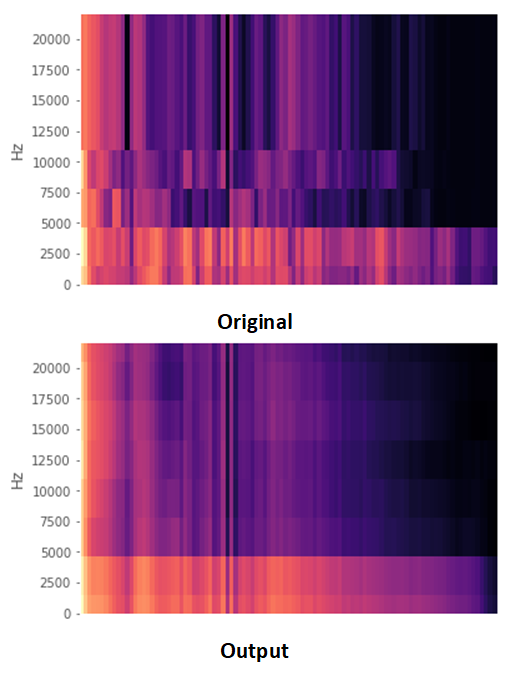
\includegraphics[width=0.2\textwidth]{figures/autoencoded.png}
    \end{center}
    \caption{The original spectrogram and the auto-encoder result after training.}
    \label{fig:encode}
\end{wrapfigure}

These experiments attempted to measure the effectiveness of different encoding approaches as well as a base case of an extracted feature vector. Audio is read in using a blocksize of 2s or 250ms with overlap of 1s and 125ms respectively. This is done to determine effective time windowing of the data, however this approach added some overhead for reading of files as summarized in Table ~\ref{tab:base-time}. A more granular blocksize causes the read and processing time to greatly increase, because of the increase in individual audio clips being evaluated.

\begin{table}[h]
    \centering
    \begin{tabular}{c|cc}
    \textbf{Window} & \textbf{Read} & \textbf{Process} \\ \hline
    250              & 7840           & 37318                    \\
    2000             & 2413           & 4831                   
    \end{tabular}
    \caption{The average read time for 400 documents and processing time by librosa. Time in ms.}
    \label{tab:base-time}
\end{table}

\subsubsection{Extracted Features}
This representation of the audio was created using feature extraction techniques found in the librosa library \cite{brian_mcfee_2018_1252297}. The features chosen for classification as a base case were the first 13 MFCCs and the spectral contrast of the signal. MFCCs are common in audio classification tasks as they are often able to keep much of the signal's information without needing the entire spectrogram. The first and second derivative of MFCCs were also computed for the feature vector to provide the learner with some features that can emulate how the signal changes over time. To this end, spectral contrast is also added as it provides the contrast between the peaks and valleys of the signal at each frame. The extracted features are then averaged down to a single vector per frame. In all, the feature vector is made up of 49 values.

\subsubsection{Neural Network}
As mentioned before, it is common to use an auto-encoder to create latent variables for classification. The idea is similar to that of a clustering algorithm like Principal Components Analysis in which the algorithm tries to find features that are of greatest variance. Here, both traditional neural networks and convolutional neural networks are used to create an encoder. The overall results were underwhelming with the biggest gain being made on the testing set. In all these auto-encoders provided about +/- 5\% accuracy change which can also be attributed to shuffling of data during training. The results of the auto-encoding with CNNs are summarized in Figure ~\ref{fig:encode}. Here, frames of audio are converted into expanded representations with more weight given to the most recent frame so the encoder can learn temporal relationships. It appears to learn a latent representation well with a reconstruction score of approximately 47\%. However, the auto-encoder takes between 45 and 75 minutes to fully train and the results are no better than previous.

\subsubsection{Classification}

\begin{table}[h]
    \begin{tabular}{lll}
        & 250ms   & 2000ms  \\ \hline
    SVM & 0.627 & 0.622 \\
    SNN & 0.717 & 0.729 \\
    RFC & 0.688 & 0.665
    \end{tabular}
    \caption{Classifier precision for top level.}
    \label{tab:topacc}
\end{table}

\begin{figure}[h]
    \centering
    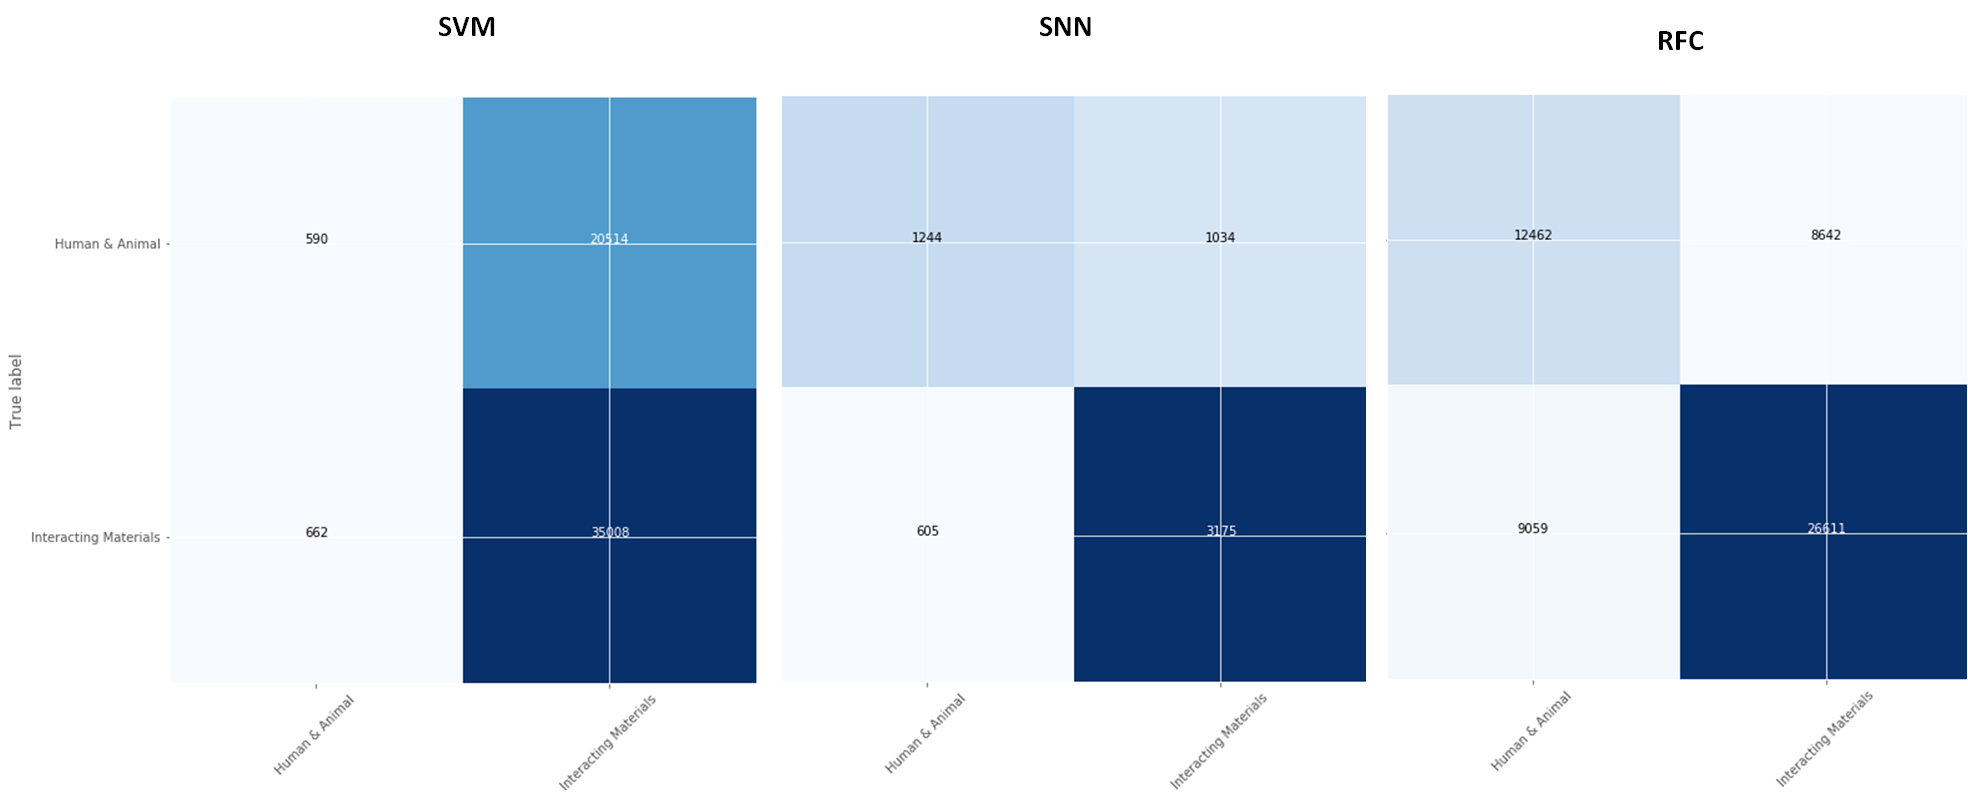
\includegraphics[width=0.45\textwidth]{figures/Top_Level_Comparison.png}
    \caption{Confusion matrices of top level classifiers.}
    \label{fig:TopClass}
\end{figure}

\subsubsection{Top Level Classifier}
As described previously, this classifier is meant to discriminate between the highest level of the Gaver taxonomy. Table ~/ref{tab:topacc} summarizes the precision of each of these classifiers for the different blocksizes. Figure ~\ref{fig:TopClass} shows the confusion matrix of the most accurate model for each classifier as there was little difference between the blocksizes. The experiments show that the shallow network approach provides the best approximation of the two classes. SVMs were the poorest performers at 63\% accuracy at maximum with most guesses being for interacting materials. In this case, it is likely that the features used for evaluation were not linearly differentiable and thus the standard SVM was unable to find a good decision boundary. RFCs and SNNs performed similar in this task with the SNN giving slightly more weight to interacting elements than the RFC.

\begin{table}[h]
    \caption{Classifier precision for \textit{Animal Voices}.}
    \label{tab:animvocprec}
    \begin{tabular}{lll}
        & 250   & 2000  \\ \hline
    SVM & 0.069 & 0.073 \\
    DNN & 0.280 & 0.300 \\
    RFC & 0.254 & 0.212
    \end{tabular}
\end{table}

\begin{figure}[b]
    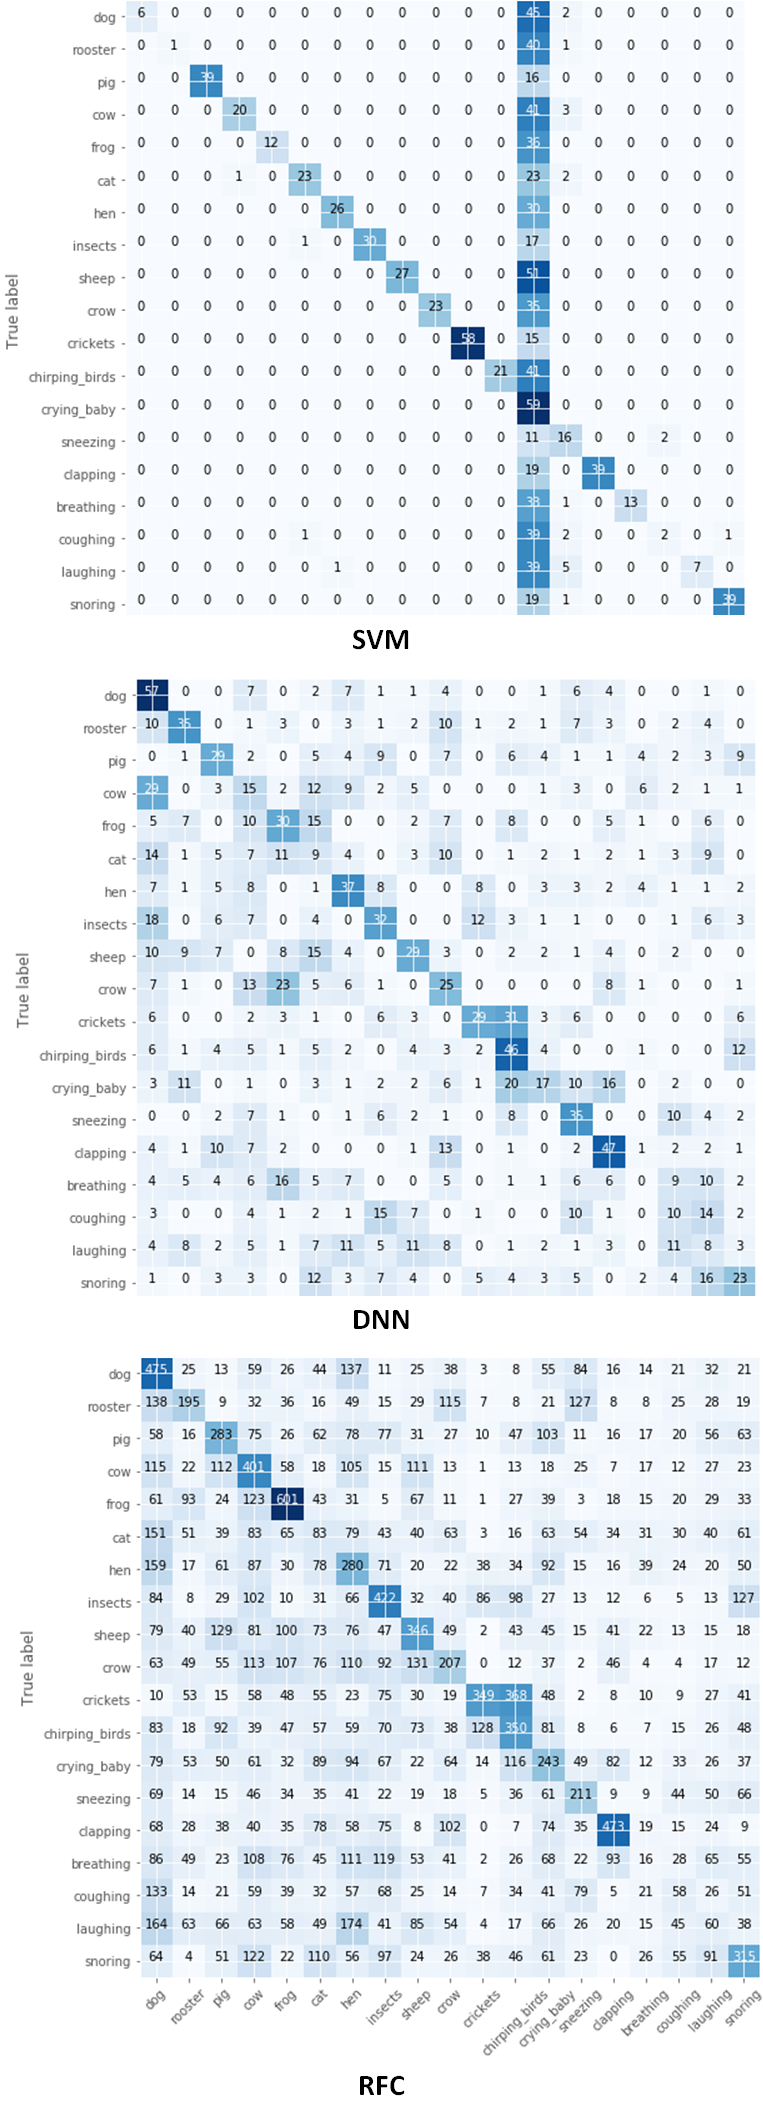
\includegraphics[width=0.35\textwidth]{figures/Animal_Classification_Comparison.png}
    \caption{Summary of classification results for the \textit{Animal Voices} classifier.}
    \label{fig:AnimClass}
\end{figure}

\subsubsection{Animal Voices Classifier}

The classifier is trained on the 19 classes identified beforehand. The 19 classes that make up the animal sounds in the dataset have some overlap, especially for identifiers like "breathing" and "laughing" as these are often breathy sounds. The precision results of each classifier is summarized in Table ~\ref{tab:animvocprec}. Here, DNNs outperform both classifiers on precision however with a 2 second time window we see DNN achieve its maximum precision while RFC precision decreases.

The confusion matrices in Figure ~\ref{fig:AnimClass} illustrates the agent often misclassifies breathing, coughing, laughing, and snoring across nearly every other class. This phenomenon is illustrated by the cutout in Figure ~\ref{fig:breath}. The highest concentration of false predictions of these four classes occurs between the classes. It is believed that this is likely due to the sounds in the dataset invariably capturing the animal's breathing patterns which, in this case, trains the network on mislabeled breathing examples.

\begin{figure}[h]
    \centering
    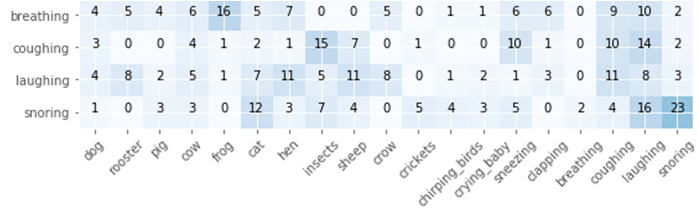
\includegraphics[width=0.45\textwidth]{figures/breathcorrelation.png}
    \caption{A cutout of the \textit{Animal Voice} DNN matrix.}
    \label{fig:breath}
\end{figure}

Another false correlation arose in this subset of the data, the agent is consistently confused between birds chirping and crickets. This is likely due to both the pitch and duration of the sounds being more similar to each other than to other sounds in the training set. This causes the agent to give less importance to these classes during training as committing neurons to them increases the loss elsewhere.

\begin{table}[h]
    \begin{tabular}{ccc}
        & 250   & 2000  \\ \hline
    SVM & 0.045 & 0.057 \\
    DNN & 0.189 & 0.191 \\
    RFC & 0.185 & 0.176
    \end{tabular}
    \caption{Classifier precision for \textit{Interacting Materials}.}
    \label{tab:interactprec}
\end{table}

\begin{figure}[h]
    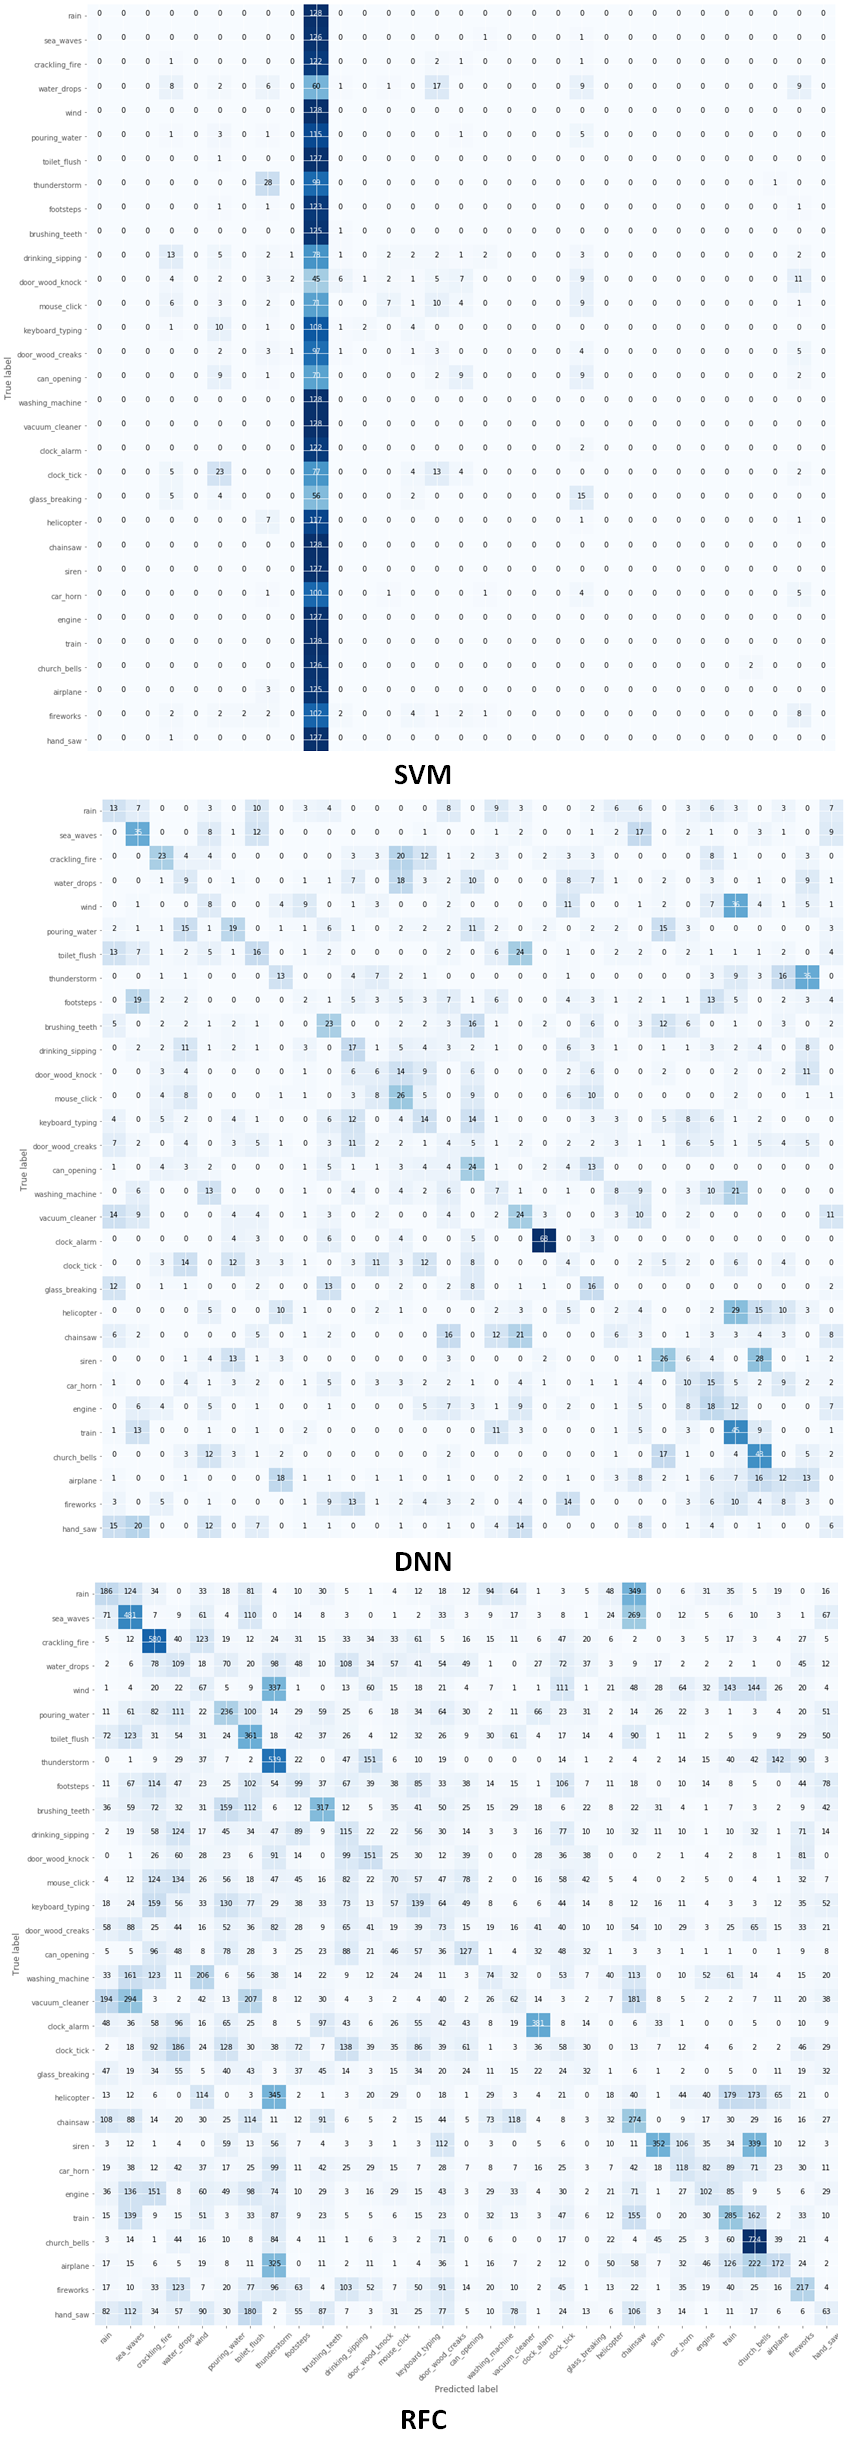
\includegraphics[width=0.35\textwidth]{figures/Material_Classification_Comparison.png}
    \caption{Summary of classification results for the \textit{Interacting Materials} classifier.}
    \label{fig:InterClass}
\end{figure}

\subsubsection{Interacting Materials}
This classification task has 31 classes, with many having overlapping kinds of sounds. This is especially true of classes with flowing water which makes up 25\% of the data. As seen in Figure ~\ref{fig:InterClass} class confusion is widespread in DNNs though it is more densely concentrated than the results of the RFC. The hypothesis is that these confusions have a basis in the source and where the sound was recorded.

In the results here we found that much of the class confusion was a result of the sound tags being ambiguous with regard to other classes. This is most apparent in classes that are in some way related to water. Here we have separate classes for pouring water, rain, sea waves, and water drops among others. The potential for confusion here is high as recordings with rain will invariably have examples of pouring water in them, similarly water drops are nearly synonymous with rain. Under this scrutiny, it is unsurprising that these classes were often confused for each other.

Related to this phenomenon in \textit{Interacting Materials} is the occurrence of recordings containing overlapping sounds found elsewhere in the dataset. An example of this is the car horn class which understandably has audio documents that have a horn honking as the car is running. Since another detection target is engine, it is possible that blocks of audio from a car horn document will be classified as an engine. While this perception is correct, it is technically incorrect in the classification task and is marked as such. This kind of confusion is mitigated through our use of probabilistic ranking in results.

\begin{table}[h]
    \centering
    \begin{tabular}{ccc}
         & 250   & 2000  \\ \hline
    DNN  & 0.174 & 0.191 \\
    HDNN & 0.246 & 0.130
    \end{tabular}
    \caption{Classification results of a hierarchical DNN and a standard DNN trained on all 50 classes.}
    \label{tab:overallprec}
\end{table}


\begin{figure}[h]
    \caption{Resultant confusion matrix of HDNN model.}
    \label{fig:Overall}
    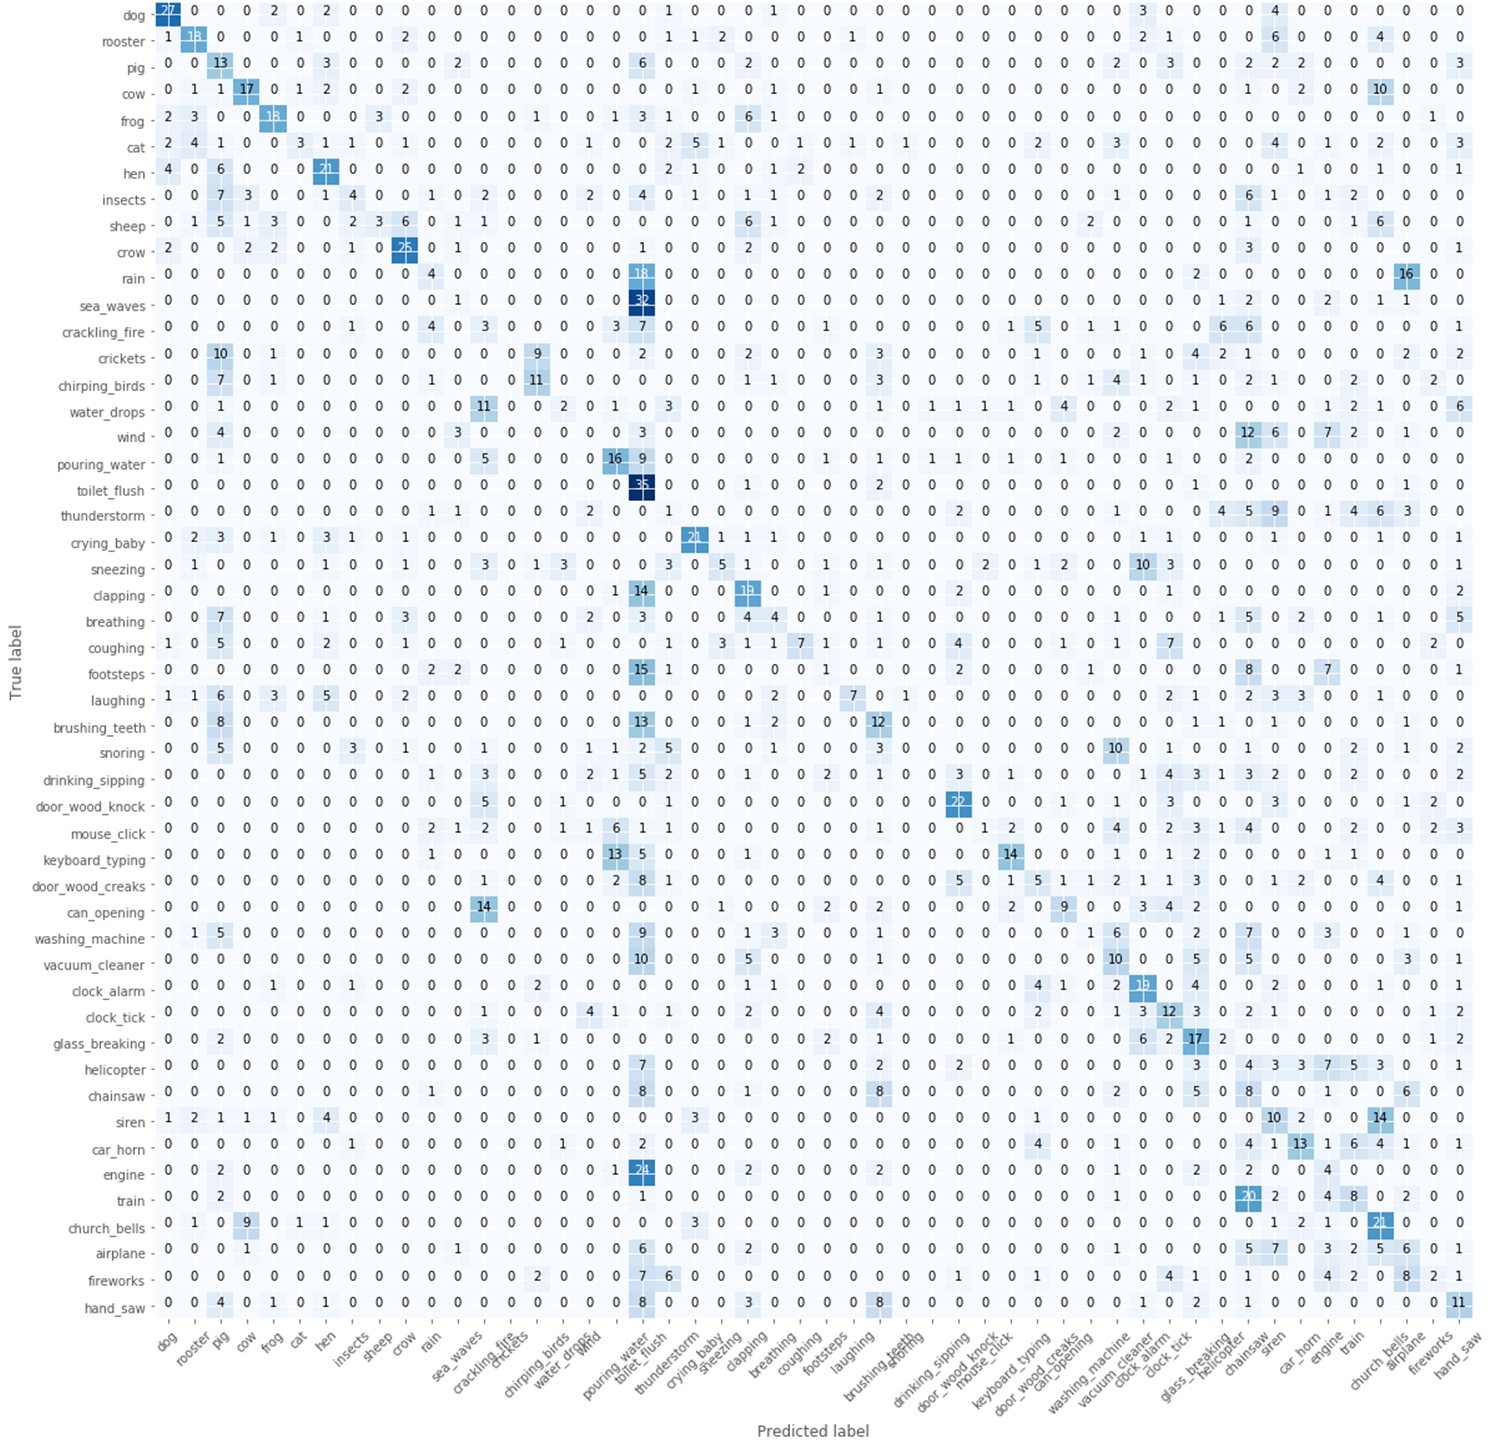
\includegraphics[width=0.40\textwidth]{figures/Overall.png}
\end{figure}

\subsubsection{Overall Accuracy}
Here, we compare a DNN trained on all 50 classes at once to the hierarchical DNN (HDNN). The class of each document in the dataset is determined in the HDNN as the highest average probability class. It is important to note that this does not mean that all frames are equally certain of the class but that a majority considered it to be the correct class. As Table ~\ref{tab:overallprec} shows, the HDNN performs better when given more granular data on which to learn. This is likely a consequence of the learner having a more focused time window to better learn audio objects individually.

Figure ~\ref{fig:Overall} illustrates a shortcoming of this prediction evaluation model. The line along the pouring water class is highly correlated to classes with water in them. It is likely that a majority of the audio document continuously has the sound of running water which is overwhelming the instances of the target class. This becomes even more clear when viewing the probability results of documents, it is often that the second-most probable class is the canonically correct class. This phenomenon is demonstrated by Figure ~\ref{fig:probChart}. In this case, it is unclear which should be taken as they have nearly equal probabilities but only one of them is technically correct. However, this is not as much of an issue when using this kind of classifier for retrieval as it is more important that a sound is detected in a document and not whether or not it is certainly the only sound in the document.

\begin{figure}[h]
    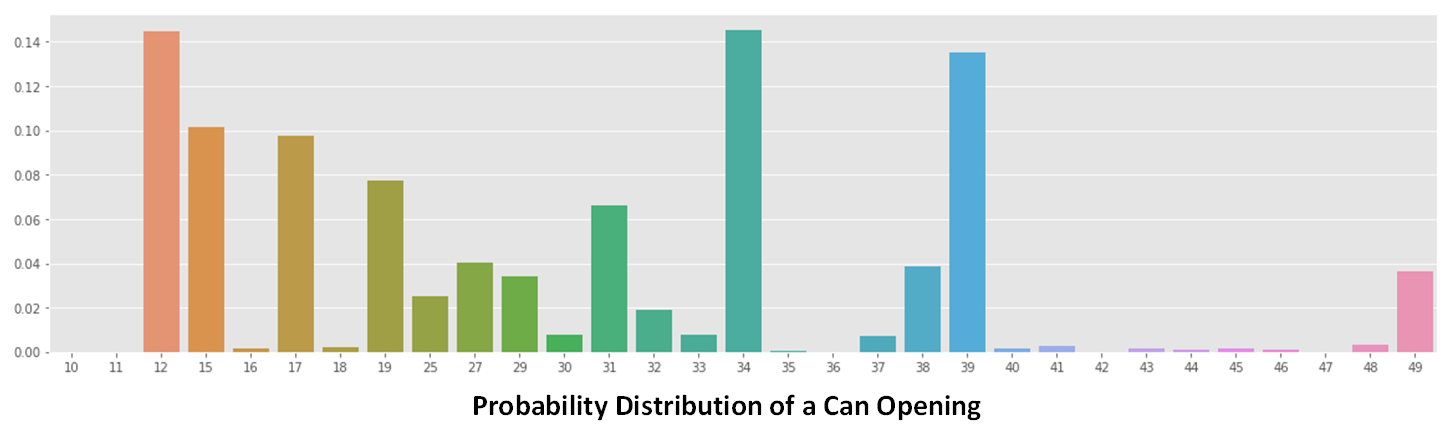
\includegraphics[width=0.50\textwidth]{figures/probchart.png}
    \caption{Probability distribution of a can opening, the target class is 34 which here is tied for first.}
    \label{fig:probChart}
\end{figure}

\section{Conclusion}
The approach here shows promise, especially in the context of a retrieval system. Using human perception as a model is an approach that had been pursued in machine vision with success and it is only logical to do the same for machine listening. By understanding the mechanisms by which we convert auditory signals to brain signals, we can understand how the audio needs to be encoded for use in machine hearing. One of the aspects of audio we have yet to optimally integrate are temporal features which are of utmost importance in audio signals.

To this end, several representations were attempted in this work. The first was just basic feature extraction from spectral representations of the audio using librosa. Librosa allowed for many spectral and temporal features to be taken from the signal though it is a slow process and may still not provide a good feature set. To better emulate human perception, auto-encoders were attempted next. The thought was that a neural network will be able to find latent variables that are of better use than those extracted from usual means. However, it was found that this approach did not bear out and hardly effected performance.

Experiments were run comparing this approach to two off-the-shelf classifiers on each layer of the hierarchy. The SVM classifier consistently under-performed and will likely be removed from subsequent evaluations. A Random Forest Classifier was consistently about equal to the neural networks it was evaluated against but in nearly every case, the network was able to beat its precision score.

Overall, this study provided insights into the complexity of autonomous audio analysis and the challenges that are still facing the field. of these challenges, it seems that representation is the most pressing. It appears though that the current direction of studying human perception mechanisms and emulating them will prove optimal.

\section{Future Work}

The hierarchical approach in its current iteration only provides minimal improvement over standard DNNs. However, the lessons learned here provide a basis on which to build out a more performant system. First, representation will be revisited and recurrent neural networks will be employed to aid in creating a new representation that considers audio's temporal nature. Second, more specific probabilistic neural networks will be investigated for integration into the \textit{Animal Voices} and \textit{Interacting Materials} classification tasks. Finally, a querying front-end will be developed for this and will be used for querying of the AudioSet dataset.